\section{Branching Ratios} \label{sec:higgs:branching}

The coupling of the SM Higgs with the gauge bosons and fermions has been shown
to give these particles their mass, however it also means that the Higgs can
decay into all of these particles.  In order of most to least likely final
states of a Higgs decay we have the decay to; a pair of $b$-quarks ($b\bar{b}$),
a pair of weak vector bosons where one is off-shell ($VV^{*}$), two gluons
($gg$), a duo of tau leptons ($\tau^{+}\tau^{-}$), or a pair of photons
($\gamma\gamma$).  Similar to the ggF production mechanism discussed in
\Cref{sec:higgs:production} the decays to massless gauge bosons (photons and
gluons) are facilitated through loops of massive particles. The exact feynman
diagrams depicting the above process' are shown in \Cref{fig:higgs_decay} while
information about their branching ratios is detailed in
\Cref{table:higgs_branching_ratios}.

\begin{figure}[!htbp]
\centering

\subcaptionbox{$H \rightarrow b\bar{b}$}{
\resizebox{0.48\textwidth}{!}{
\begin{tikzpicture}[thick]
 \begin{feynman}
  \vertex (origin);
  \vertex [right=1.5cm of origin] (H);
  \vertex [above right=0.50cm and 1.5cm of H] (b1) {\(\bar{b}\)};
  \vertex [below right=0.50cm and 1.5cm of H] (b2) {\(b\)};
  \diagram* {
  (origin) -- [red, scalar, edge label={\(H\)}] (H),
  (b1) -- [fermion] (H) -- [fermion] (b2),
  };
 \end{feynman}
\end{tikzpicture}
}}
\subcaptionbox{$H \rightarrow W^{\pm}W^{\mp*}$}{
\resizebox{0.48\textwidth}{!}{
\begin{tikzpicture}[thick]
 \begin{feynman}
  \vertex (origin);
  \vertex [right=1.5cm of origin] (H);
  \vertex [above right=0.50cm and 1.5cm of H] (W1) {\(W^{\pm}\)};
  \vertex [below right=0.50cm and 1.5cm of H] (W2) {\({W^{\mp}}^{*}\)};
  \diagram* {
  (origin) -- [red, scalar, edge label={\(H\)}] (H),
  (W1) -- [boson] (H),
  (W2) -- [boson] (H),
  };
 \end{feynman}
\end{tikzpicture}
}} \\
\subcaptionbox{$H \rightarrow gg$}{
\resizebox{0.48\textwidth}{!}{
\begin{tikzpicture}[thick]
 \begin{feynman}
  \vertex (origin);
  \vertex [right=1.5cm of origin] (H);
  \vertex [above right=1cm and 1.2cm of H] (v1);
  \vertex [below right=1cm and 1.2cm of H] (v2);
  \vertex [right=1.75cm of v1] (g1) {\(g\)};
  \vertex [right=1.75cm of v2] (g2) {\(g\)};
  \diagram* {
  (origin) -- [red, scalar, edge label={\(H\)}] (H),
  (H) -- [fermion] (v1) -- [fermion] (v2) -- [fermion] (H),
  (g1) -- [gluon] (v1),
  (g2) -- [gluon] (v2),
  };
 \end{feynman}
\end{tikzpicture}
}}
\subcaptionbox{$H \rightarrow \tau^{+}\tau{-}$}{
\resizebox{0.48\textwidth}{!}{
\begin{tikzpicture}[thick]
 \begin{feynman}
  \vertex (origin);
  \vertex [right=1.5cm of origin] (H);
  \vertex [above right=0.50cm and 1.5cm of H] (tau1) {\(\tau^{+}\)};
  \vertex [below right=0.50cm and 1.5cm of H] (tau2) {\(\tau^{-}\)};
  \diagram* {
  (origin) -- [red, scalar, edge label={\(H\)}] (H),
  (tau1) -- [fermion] (H) -- [fermion] (tau2),
  };
 \end{feynman}
\end{tikzpicture}
}} \\
\subcaptionbox{$H \rightarrow ZZ^{*}$}{
\resizebox{0.48\textwidth}{!}{
\begin{tikzpicture}[thick]
 \begin{feynman}
  \vertex (origin);
  \vertex [right=1.5cm of origin] (H);
  \vertex [above right=0.50cm and 1.5cm of H] (Z1) {\(Z\)};
  \vertex [below right=0.50cm and 1.5cm of H] (Z2) {\(Z^{*}\)};
  \diagram* {
  (origin) -- [red, scalar, edge label={\(H\)}] (H),
  (Z1) -- [boson] (H),
  (Z2) -- [boson] (H),
  };
 \end{feynman}
\end{tikzpicture}
}}
\subcaptionbox{$H \rightarrow \gamma\gamma$}{
\resizebox{0.48\textwidth}{!}{
\begin{tikzpicture}[thick]
 \begin{feynman}
  \vertex (origin);
  \vertex [right=1.5cm of origin] (H);
  \vertex [above right=1cm and 1.2cm of H] (v1);
  \vertex [below right=1cm and 1.2cm of H] (v2);
  \vertex [right=1.75cm of v1] (gamma1) {\(\gamma\)};
  \vertex [right=1.75cm of v2] (gamma2) {\(\gamma\)};
  \diagram* {
  (origin) -- [red, scalar, edge label={\(H\)}] (H),
  (H) -- [fermion] (v1) -- [fermion] (v2) -- [fermion] (H),
  (gamma1) -- [photon] (v1),
  (gamma2) -- [photon] (v2),
  };
 \end{feynman}
\end{tikzpicture}
}}


\caption{Feynman diagrams representing the leading Higgs decay channels.}

\label{fig:higgs_decay}
\end{figure}

\begin{table}[htpb]
 \centering
 \caption{ The branching ratios and the relative uncertainty for a Standard Model Higgs boson with $m_{H}=125~\GeV$ \cite{PDG2018:Ch11}.}
 \begin{tabular}{@{}lrr@{}} \toprule
  Decay Channel           & Branching Ratio       & Relative Uncertainty \\ \midrule
  $H\to b\bar{b}$         & $5.84 \times 10^{-1}$ & $_{-3.3\%}^{+3.2\%}$ \\
  \addlinespace[0.3em]
  $H\to W^{+}W^{-}$       & $2.14 \times 10^{-1}$ & $_{-4.2\%}^{+4.3\%}$ \\
  \addlinespace[0.3em]
  $H\to \tau^{+}\tau^{-}$ & $6.27 \times 10^{-2}$ & $_{-5.7\%}^{+5.7\%}$ \\
  \addlinespace[0.3em]
  $H\to ZZ$               & $2.62 \times 10^{-2}$ & $_{-4.1\%}^{+4.3\%}$ \\
  \addlinespace[0.3em]
  $H\to \gamma\gamma$     & $2.27 \times 10^{-3}$ & $_{-4.9\%}^{+5.0\%}$ \\
  \addlinespace[0.3em]
  $H\to Z\gamma$          & $1.53 \times 10^{-3}$ & $_{-8.9\%}^{+9.0\%}$ \\
  \addlinespace[0.3em]
  $H\to \mu^{+}\mu^{-}$   & $2.18 \times 10^{-4}$ & $_{-5.9\%}^{+6.0\%}$ \\
  \bottomrule
 \end{tabular}\label{table:higgs_branching_ratios}
\end{table} 

In \Cref{table:higgs_branching_ratios} the order is determined by two distinct effects; 
the proportionality of the Higgs couplings to the mass of the decay product, and whether 
or not the rest mass of the higgs is sufficient to produce the two final state objects.  
In \Cref{fig:higgs_decay_plot} you can see that as the mass of the higgs boson gets 
closer to $2m_W$ the cross section for $H \rightarrow WW$ grows.

\begin{figure}[!htbp]
  \begin{center}
    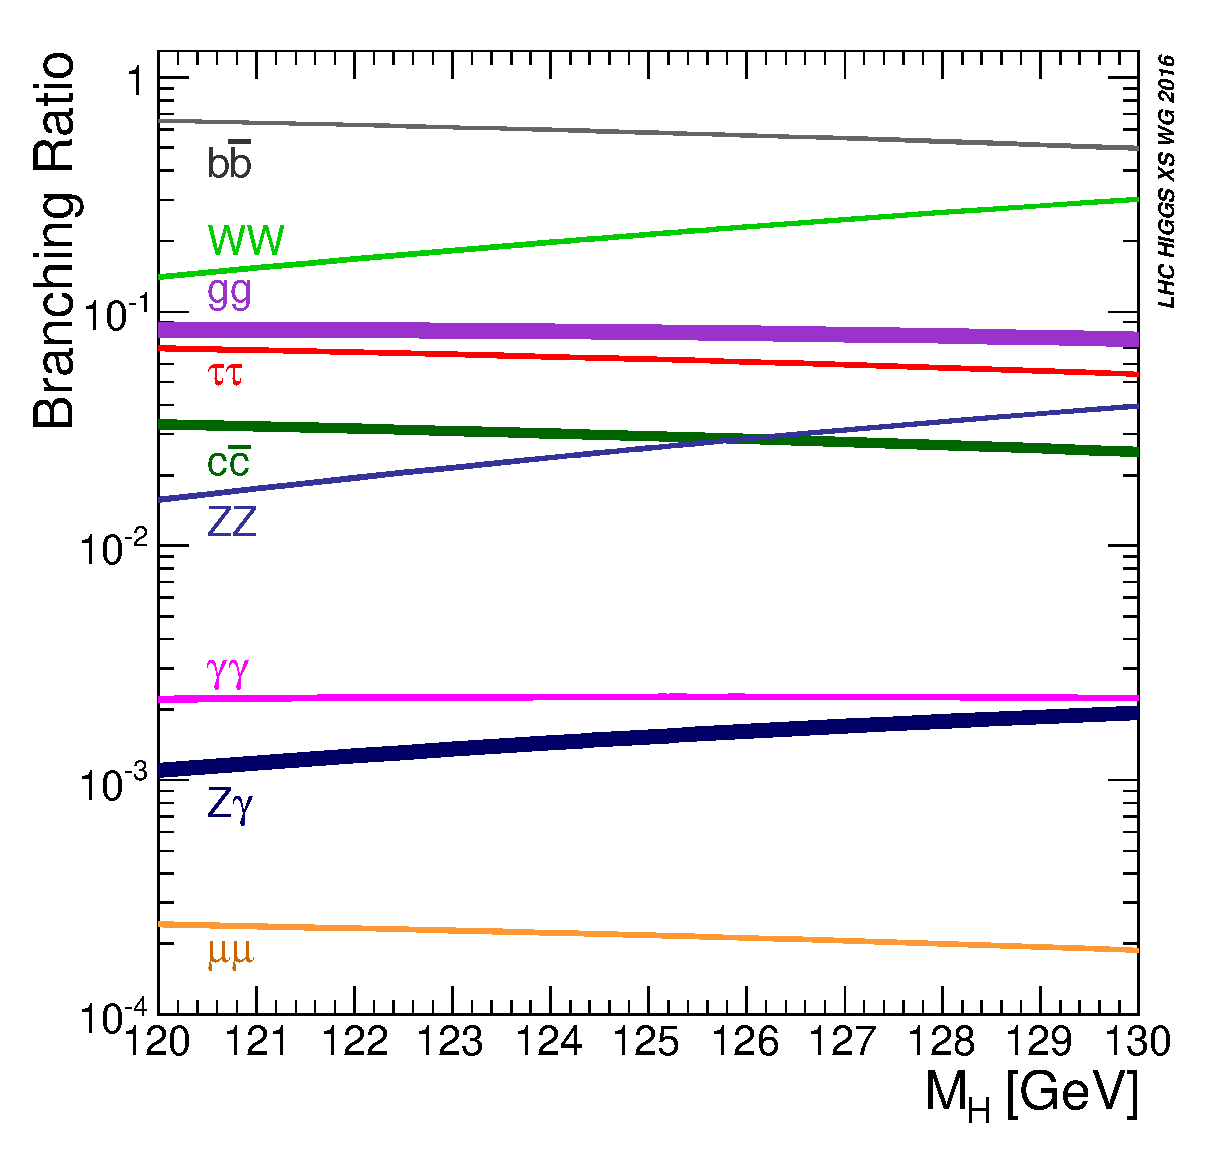
\includegraphics[width=0.5\linewidth]{figures/higgs/higgs_decay_plot.eps}
    \caption{Branching ratios for the decay of the SM Higgs boson near $m_{H} = 125$GeV including theoretical uncertainty bands \cite{PDG2018:Ch11}}
    \label{fig:higgs_decay_plot}
  \end{center}
\end{figure}


